% ! TEX root = ../mechanics.tex
\chapter{导弹的气动布局}
\section{火箭弹稳定装置的基本类型}
\begin{equation*}
  \color{titleblue}
  两种尾翼
  \begin{cases}
    弧形张开式尾翼
    \begin{cases}
      整流罩\\ 
      弧形翼片\\ 
      连接轴\\ 
      同步环
    \end{cases}\\ 
    刀形张开式尾翼
    \begin{cases}
      尾翼座\\ 
      刀形翼片
      \begin{cases}
            前张式\\ 
            后张式
          \end{cases}\\ 
      翼片转轴
    \end{cases}
  \end{cases}
\end{equation*}
\begin{equation*}
  \color{titleblue}
  尾翼的分类
  \begin{cases}
    按尾翼刚度分
    \begin{cases}
      刚性尾翼\\ 
      弹性尾翼
    \end{cases}\\ 
    按尾翼尺寸和弹径关系分
    \begin{cases}
      同口径尾翼\\ 
      超口径尾翼
    \end{cases}\\ 
    按翼片和弹体的联接方式分
    \begin{cases}
      固定式尾翼\\ 
      张开式尾翼
    \end{cases}\\ 
    按尾翼平面形状分
    \begin{cases}
      矩形尾翼\\ 
      梯形尾翼\\ 
      三角形尾翼\\ 
      刀形尾翼
    \end{cases}
  \end{cases}
\end{equation*}
\begin{notice}
两种尾翼的特点
\begin{enumerate}
  \item 弧形张开式尾翼
    \begin{enumerate}
      \item 平时合拢在弹体上,最大外径不超过
        弹体直径,结构紧凑.
      \item 四片尾翼同时张开
      \item 翼片弧长最大不能超过弹体的$\frac{1}{4}$
        周长,为提供足够升力必须加大弦向尺寸.
      \item 翼片根部容易出现强度不足的问题.
    \end{enumerate}
  \item 刀形张开式尾翼
    \begin{enumerate}
      \item 翼片张开动力可选弹簧力,弹体自旋离心力等
      \item 能充分利用弹上的空间.
      \item 展向尺寸较大,为提高强度需加厚,阻力较大.
    \end{enumerate}
\end{enumerate}
\end{notice}

\subsection{尾翼的几何参数}
{\bfseries 展长}\index{展长}指机翼左右翼尖之间的距离.

{\bfseries 弦长}\index{弦长}指机翼前缘到机翼后缘之间的
距离.

{\bfseries 后掠角}\index{后掠角}指机翼设计中心线和机身
之间的夹角.

尾翼的主要参数包括{\color{blue}展弦比$\lambda$,后
掠角$\chi$,根稍比$\eta$,相对厚度$\overline{c}$,翼片
数$N$以及剖面形状}.

\begin{notice}
翼面参数的影响
\begin{enumerate}
  \item 展弦比:\\ 
    对亚音速飞行的火箭弹,增大展弦比可以减小阻力;当
    火箭弹超音速飞行时,增大展弦比会增大阻力.
  \item 后掠角:\\ 
    后掠角的作用时提高翼面的临界马赫数,以延缓前缘波
    阻的产生,从而有效的降低尾翼阻力系数的值.后掠角
    越大,临界马赫数就越大,火箭弹在低超音速飞行时,
    激波出现的可能性就越小,从而阻力减小.
  \item 根稍比:\\ 
    根稍比对气动力影响不显著.根稍比大的尾翼,气动载荷
    分布更靠近根部.梯形尾翼和三角翼气动性能差异小,但
    梯形尾翼翼尖刚度高.
  \item 相对厚度:\\ 
    尾翼的相对厚度主要影响阻力.厚度增加,阻力总是增加的.
    在保证强度,刚度条件下,应尽可能减小相对厚度.
  \item 剖面形状:\\ 
    剖面形状主要影响厚度波阻.选择翼剖面形状时,既要
    考虑尾翼的气动特性,又要考虑强度,刚度及加工工艺
    特性.
  \item 翼片数量:\\ 
    尾翼段阻力系数与翼片对数成正比,而增加$N$时,升力
    系数增加较小.
\end{enumerate}
\end{notice}
{\color{blue}
\begin{itemize}
  \item 减小展弦比,增加根稍比,可以使尾翼结构质量降低.
  \item 减小相对厚度,对实心结构的翼剖面来说,可以使
    尾翼的质量降低.
\end{itemize}}
在设计尾翼时,满足结构设计和飞行稳定性的条件下,应采用
小展弦比,大根稍比,小相对厚度.
\section{导弹的气动外形}
有翼导弹的升力,控制力主要由弹身,翼面,舵面产生.

  翼面沿周向的配置如下图
\begin{figure}[!ht]
  \centering 
  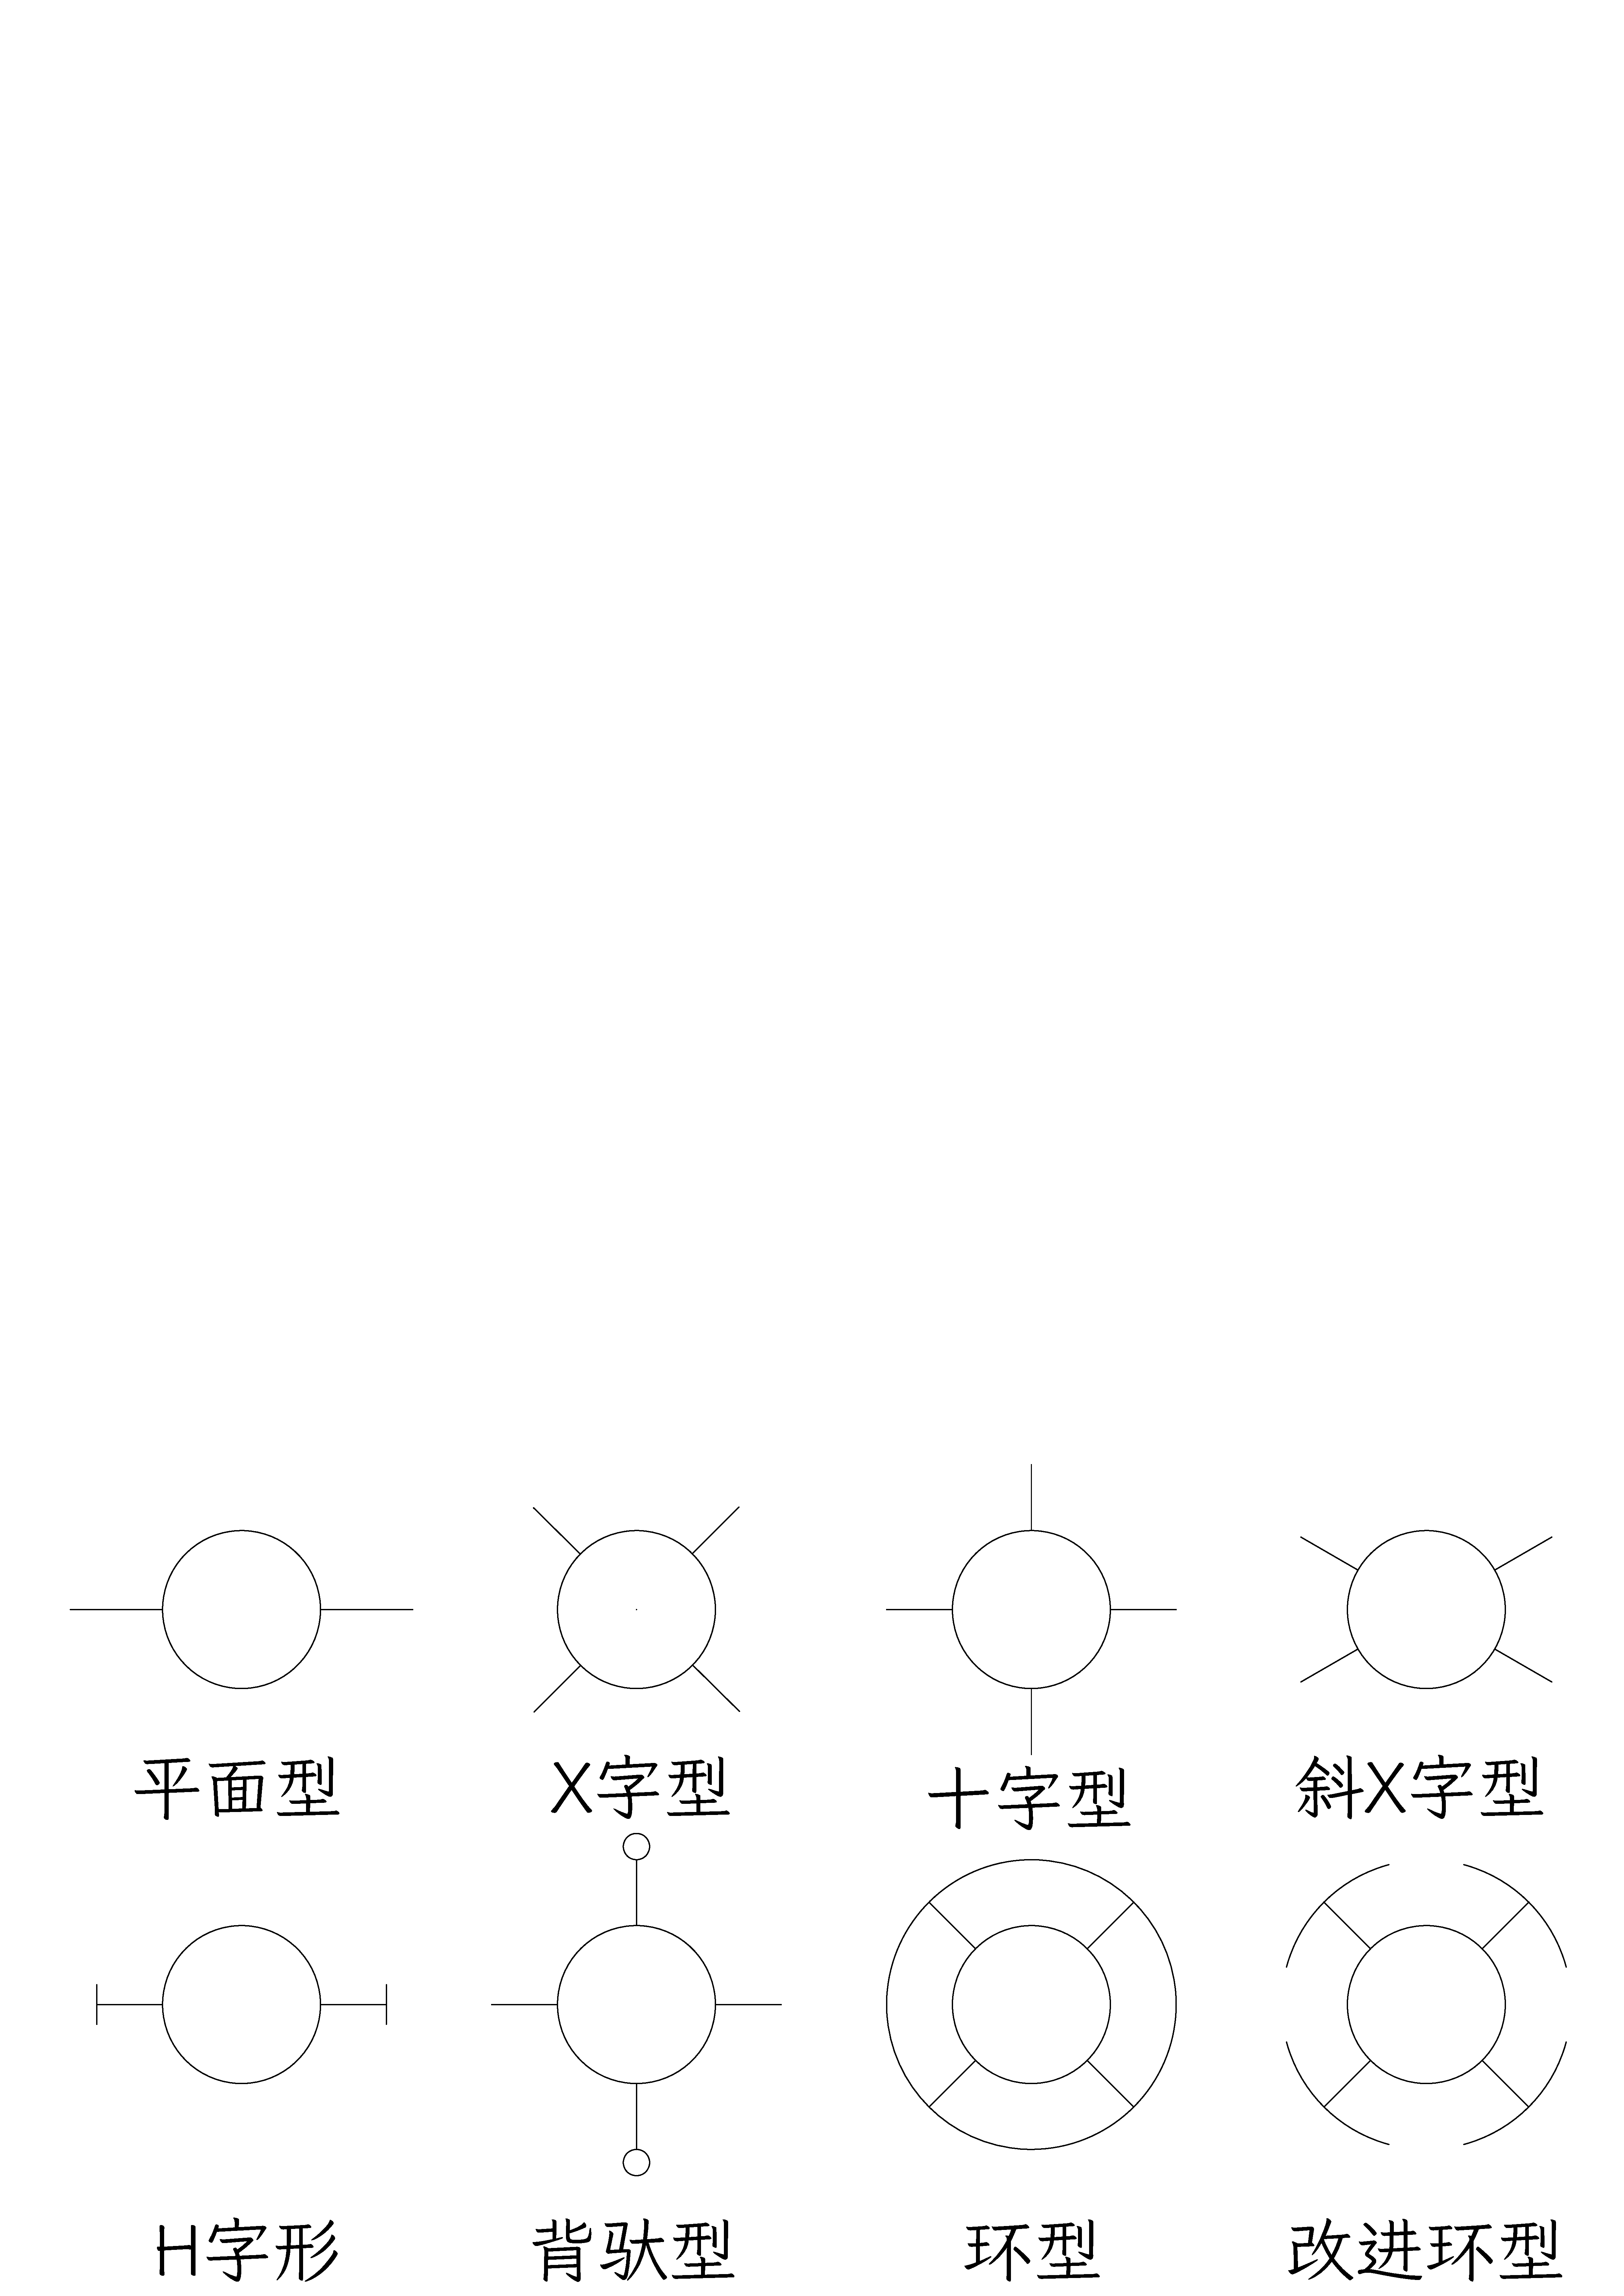
\includegraphics[width=9cm]{./Introduction_to_rocket_missile_tec/wings.pdf}
\end{figure}

\begin{equation*}
  \color{titleblue}
  翼面沿弹身轴向的布局
  \begin{cases}
    正常式\text{:}弹翼在前,操纵面在后\\ 
    鸭式\text{:}弹翼在后,操纵面在前\\ 
    旋转弹翼式\text{:}弹翼在前,同时又是
    操纵面:固定尾翼在后,起稳定作用\\ 
    无尾式\text{:}操纵面位于弹翼的后缘\\ 
    无弹翼式\text{:}尾部是操纵面,升力依靠
    弹身产生
  \end{cases}
\end{equation*}
\begin{notice}
翼面沿弹身纵向配置型式与控制特点:
\begin{enumerate}
  \item 正常式布局:\\ 
    正常式布局弹翼配置在弹身中段,舵面处于弹身
    尾段,且两组翼面通常为X-X型配置.

    条形翼可以利用翼体干扰提升升力,减质减阻.
    压心变化小,翼展小.

    特点是:
    \begin{enumerate}
      \item 由于舵面负偏转角产生一个使头部上抬的力矩
        ,所以舵面偏转角和弹体攻角相反.舵面产生的控制力
        的方向也始终与弹体攻角产生的升力方向相反,导弹的
        响应特性比较差.
      \item 升力特性和响应特性较鸭式布局和全动翼要差.
      \item 弹翼固定不偏转,空气动力的线性程度较其他两种
        布局要好些.
    \end{enumerate}
  \item 无翼式布局:\\ 
    实际就是全动翼式,整个弹翼做成可转动的.既可起翼的作用,
    又可以起舵的作用.可以提供很大的法向力(大机动过载).
    
    特点是:
    \begin{enumerate}
      \item 具有需要的过载特性
      \item 大大改善了非对称气动力特性
      \item 具有较高的舵面效率和需要的纵向静稳定性
      \item 具有较轻的质量和较小的气动阻力
      \item 结构简单,操作方便,使用性能好
    \end{enumerate}
  \item 鸭式布局:\\ 
    翼面布局与正常式相反,小的舵面位于弹身前部,大的弹翼
    位于弹身中后部.
    
    特点是:
    \begin{enumerate}
      \item 鸭式舵偏转方向始终与攻角一致,故其升阻比大
      \item 舵直接提供升力,反应快
      \item 舵在前部,舵面效率高
      \item 舵面与安定翼远离质心,便于静稳定度的调整
      \item 舵面展小,面积小,对后翼面下洗流影响小
      \item 舵面产生的升力近乎被安定翼由于舵面下洗
        而减小的升力相抵消,全弹的升力与舵面升力无关
      \item 鸭式舵{\color{red}很难作滚动控制}
    \end{enumerate}
    很难作滚动控制的解决方法是:
    \begin{enumerate}
      \item 减小尾翼翼展,以减小反滚转力矩
      \item 采用环形尾翼
      \item 采用新型的自由旋转尾翼
      \item 环形翼的基础上,采用T型翼片组合尾翼的布局
      \item 近距离耦合式鸭式布局(P119页)
      \item 断牙形前缘鸭式舵布局(P119页)
    \end{enumerate}
  \item 旋转弹翼布局:\\ 
    弹翼旋转,起控制舵的作用.尾翼固定,起稳定翼的作用.
    法向力主要靠旋转翼提供,升力靠弹翼偏转直接产生.
    质心位于升力作用点后,质心位置最有利.
  \item 无尾式布局:\\ 
    见P122页
\end{enumerate}
\end{notice}

导弹总体设计的核心是{\color{blue}外形设计和
气动力设计}.

导弹外形设计的两个任务:
\begin{enumerate}
  \item 导弹各部件的几何参数选择及几何尺寸的计算与确定
  \item 对弹上各部件进行气动布局,合力确定各部件的位置
    与布局形式
\end{enumerate}

气动布局的要求:
\begin{enumerate}
  \item 满足导弹战术技术指标和弹上各系统工作
    要求
  \item 充分利用最佳翼身干扰和翼面间干扰以及
    外挂物与翼身的干扰,设计出最优升阻比的外形
    配置
  \item 在作战空域内,导弹要满足机动性,稳定性
    和操纵性的要求
  \item 保证在最大使用攻角范围内,空气动力学
    特性尽可能处于线性范围,尤其是力矩特性
  \item 气动控制面设计要保证在使用攻角和速度
    范围内,压心变化尽可能小
  \item 便于运输,贮存和实战使用
\end{enumerate}

